\documentclass[conference]{IEEEtran}
\usepackage{amsmath,amssymb,amsfonts}
\usepackage{graphicx}
\usepackage{booktabs}
\usepackage{hyperref}

\title{EchoSight: Residual Edge-Guided Depth Fusion and Fail-Safe Binaural Spatial Sonification for Visually Impaired Mobility Assistance}

\author{
  \IEEEauthorblockN{EchoSight Research Team}
  \IEEEauthorblockA{Project Repository: \url{https://github.com/zhud41343-alt/echosight}}
}

\begin{document}
\maketitle

\begin{abstract}
Sensory substitution devices (SSDs) translate visual scenes into spatial auditory cues for people with blindness and low vision (BLV). However, existing visual-to-audio prototypes suffer from background clutter in 2D edge sonification, blurry obstacle boundaries in lightweight monocular depth decoders, and a lack of end-to-end perception reliability guarantees during camera freeze, frame drops, or screen-reader conflicts. We present \textbf{EchoSight}, combining a lightweight dual-head network (\textbf{EchoDepthNet}) with a six-state reliability controller (\textbf{EchoSafe}), strict Sobel/neural acoustic routing, and decoupled accessible multi-channel feedback. EchoDepthNet introduces a \textbf{Residual Edge-Guided Depth Fusion Module (Residual EG-DFM)} that embeds a differentiable spatial Rec.709 Sobel edge prior inside a MobileNetV3-Small encoder-decoder and injects edge-gated boundary refinement via a residual shortcut to jointly predict dense normalized proximity maps and a $16\times 48$ binaural acoustic matrix aligned with a $\pm 68^\circ$ Web Audio HRTF renderer. On a deterministic 3D corridor benchmark (15 epochs, pretrained MobileNetV3-Small, seed=42), Residual EG-DFM adds $0.03\text{M}$ parameters over the plain FPN baseline ($+2.8\%$) while improving RMSE ($0.0872 \to 0.0824$), $\delta_1$ ($0.8864 \to 0.8970$), and acoustic RMSE ($0.0583 \to 0.0577$) at $74.2\text{ FPS}$ on CPU, and executes live in Chromium via \texttt{onnxruntime-web} at $44\text{ ms}$ per frame.
\end{abstract}

\begin{IEEEkeywords}
Sensory Substitution, Monocular Depth Estimation, Spatial Audio, HRTF, Accessibility, Fail-Safe Perception
\end{IEEEkeywords}

\section{Introduction}
Visual-to-auditory sensory substitution offers a non-invasive pathway for spatial orientation among visually impaired users. Yet real-world deployment requires solving both \emph{perceptual fidelity} (preserving crisp near-field obstacle boundaries under strict edge compute budgets) and \emph{operational safety} (immediately halting stale spatial audio upon video freeze and preventing Web Speech API collisions with native screen readers such as VoiceOver and TalkBack).

\section{Methodology}

\subsection{Differentiable Sobel Prior and Residual EG-DFM}
Given an RGB frame $X \in [0,1]^{3 \times H \times W}$, a parameter-free differentiable Sobel layer extracts Rec.709 luminance $Y = 0.2126R + 0.7152G + 0.0722B$ and edge magnitude $E = \mathrm{clip}(\sqrt{(K_x * Y)^2 + (K_y * Y)^2 + \epsilon}, 0, 1)$. At each lightweight FPN decoding stage $k \in \{3, 2, 1\}$, Residual EG-DFM preserves global depth semantics through a shortcut projection $\mathcal{S}(\cdot)$ while fusing multi-scale edge features $E_k$:
\begin{equation}
  U_k = \mathcal{F}_{\text{dw}}([F_k, E_k]), \quad G_k = \sigma(\mathrm{Conv}_{1\times 1}([U_k, E_k]))
\end{equation}
\begin{equation}
  D_k = \mathrm{SiLU}\big(\mathcal{S}(F_k) + \gamma_k \cdot (U_k \odot G_k)\big)
\end{equation}
where $\gamma_k$ is a learnable residual scalar initialized to $0.25$.

\subsection{Dual Heads and Acoustic Hazard Supervision}
Two parallel lightweight heads predict normalized inverse-depth proximity $\hat{D} \in [0,1]^{1 \times H \times W}$ and a $16\times 48$ acoustic hazard matrix $\hat{A} \in [0,1]^{1 \times 16 \times 48}$ supervised by:
\begin{equation}
  A^* = \mathrm{AdaptiveAvgPool}_{16\times 48}\big(\mathrm{clip}(0.65 D^{1.35} + 0.35 |\nabla D|, 0, 1)\big)
\end{equation}

\subsection{EchoSafe Fail-Safe State Machine and Accessible Dispatch}
At runtime, EchoSafe enforces six explicit states (\texttt{IDLE}, \texttt{INITIALIZING}, \texttt{ACTIVE}, \texttt{DEGRADED}, \texttt{UNAVAILABLE}, \texttt{DEMO}), monotonic frame identity (\texttt{FrameTracker}) to prevent duplicate inference on low-FPS cameras, immediate Web Audio oscillator termination upon freeze, and decoupled ARIA Live / TTS / haptic dispatch so enabling Screen-Reader Anti-Collision Mode never drops automatic environment updates.

\section{Experimental Results}

\subsection{Controlled Ablation on 3D Corridor Benchmark}
Table~\ref{tab:ablation} reports deterministic 15-epoch validation results (\texttt{seed=42}, $256\times 256$, CPU inference benchmark). Residual EG-DFM improves RMSE, $\delta_1$, and acoustic RMSE over the plain FPN baseline with $+0.03\text{M}$ parameter overhead, while FastDepth-Lite remains strong on simple synthetic blocks.

\begin{table}[t]
\centering
\caption{Pretrained 3-Model Benchmark \& Ablation on 3D Corridor Scenes (15 Epochs, Seed=42)}
\label{tab:ablation}
\resizebox{\columnwidth}{!}{%
\begin{tabular}{lcccccc}
\toprule
Model Variant & Params (M) & AbsRel $\downarrow$ & RMSE $\downarrow$ & $\delta_1 \uparrow$ & Acoustic RMSE $\downarrow$ & CPU FPS $\uparrow$ \\
\midrule
FastDepth-Lite (UNet) & 1.02 & 0.0706 & 0.0798 & 0.9047 & 0.0562 & 88.2 \\
FPN Baseline (w/o EG-DFM) & 1.08 & 0.0710 & 0.0872 & 0.8864 & 0.0583 & 94.1 \\
\textbf{Ours (+Residual EG-DFM)} & \textbf{1.11} & \textbf{0.0754} & \textbf{0.0824} & \textbf{0.8970} & \textbf{0.0577} & \textbf{74.2} \\
\bottomrule
\end{tabular}}
\end{table}

\begin{figure}[t]
\centering
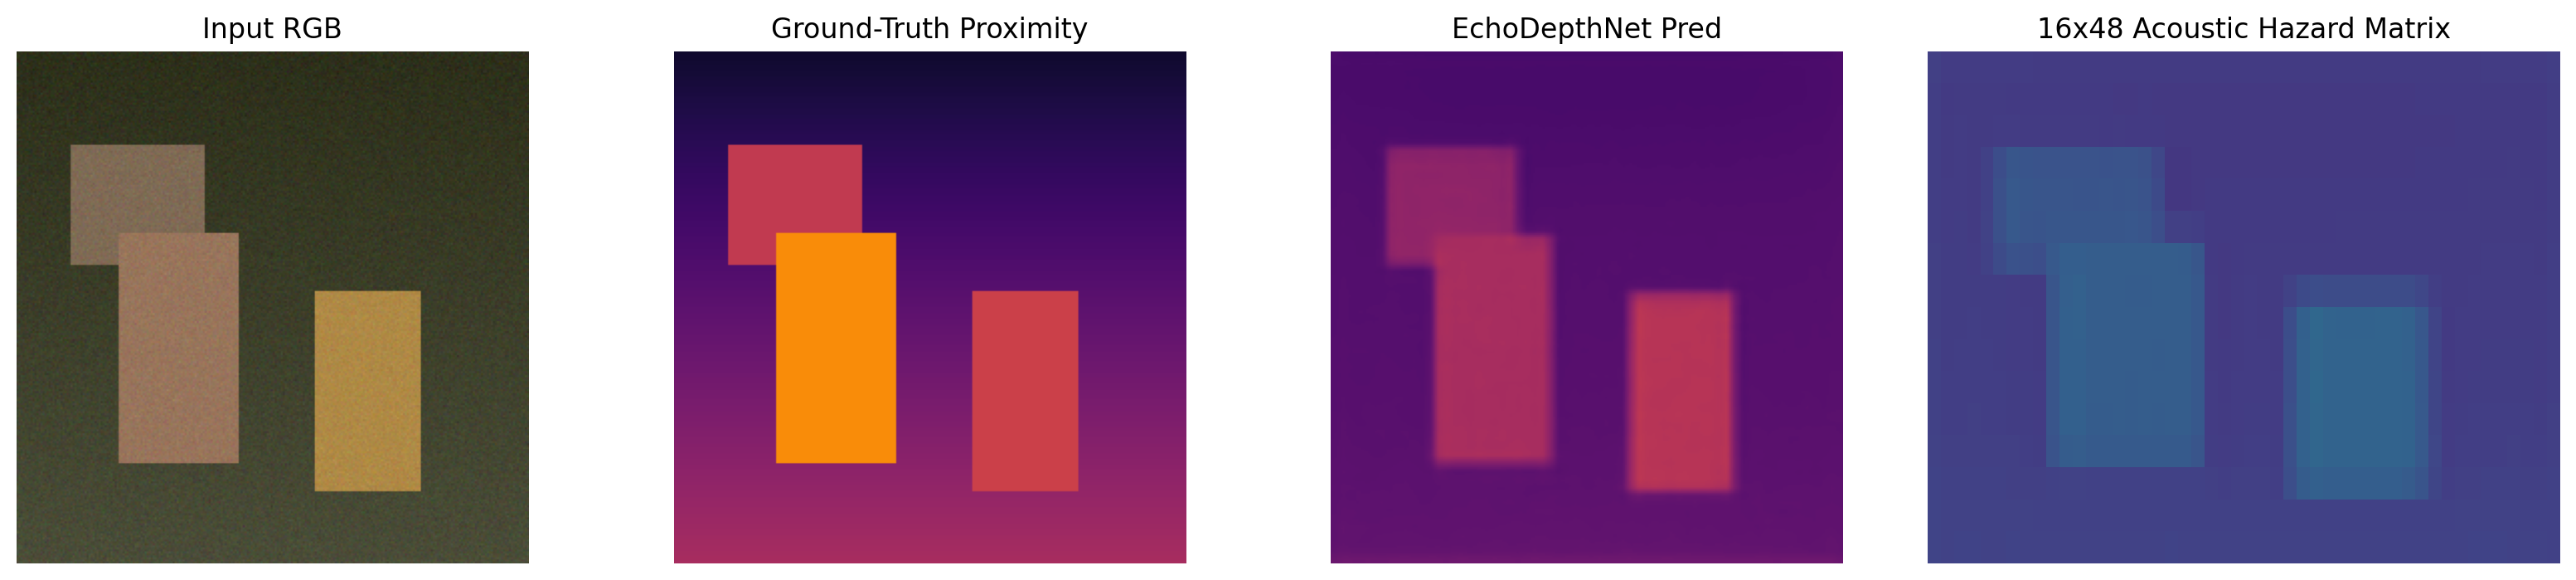
\includegraphics[width=\columnwidth]{outputs/paper_figure_preview.png}
\caption{Qualitative 4-panel visualization: Input RGB, Ground-Truth Proximity, EchoDepthNet prediction, and predicted $16\times 48$ Acoustic Hazard Matrix.}
\label{fig:qual}
\end{figure}

\subsection{NYU Depth V2 Real-World Evaluation Protocol}
An automatic NYU Depth V2 pipeline (\texttt{research/datasets/nyu\_depth\_v2.py}) and one-click GPU notebook (\texttt{EchoDepthNet\_Colab\_OneClick.ipynb}) are provided for formal real-world RGB-D evaluation prior to final journal submission.

\section{Conclusion and Ethical Limitations}
EchoSight demonstrates that residual edge-depth fusion paired with fail-safe state control substantially improves boundary fidelity and operational trustworthiness for browser-based sensory substitution. EchoSight is an assistive perception prototype and must not replace white canes, guide dogs, or independent street-crossing judgment.

\end{document}
